\chapter{Experiment}\label{ch:exp}
The experimental procedure is explained in Section \ref{sec:exp.proc}. 
It is discussed what experiments can be done in order to investigate closed-loop stability and the tracking performance of Nonlinear Geometric Control.
In addition, a comparison will be made between the performances of the Nonlinear Geometric Controller and a linear \a{lqr} controller.

The controllers are tested on their ability to track a desired load trajectory. 
Section \ref{sec:exp.traj} presents several desired load trajectories that create different challenges, and it is discussed what could be expected from these experiments.
%in what way a comparison can be made between the performance of the controllers.
%ADD 1 wat brengt mij tot keuze trajectories 
%ADD 2 trajectories
%ADD 3 waar ga ik de resultaten op checken

In Section \ref{sec:exp.setup} the experimental setup is discussed. 
The model parameters for the \a{qr}-Load system are presented, as well as the controller parameters for both Nonlinear Geometric controller and \a{lqr} controller.
The notion of a backstepping command filter is made to explain a mathematical simplification in the experiments.

Finally, in Section \ref{sec:set.results} the results that are obtained from the load trajectory tracking experiments are presented and discussed.
The stability of the closed-loop system is demonstrated for the Nonlinear Geometric Controller and the differences in linear- and nonlinear controller performance are discussed.

\newpage
\section{Procedure}\label{sec:exp.proc}
Performance of both Nonlinear Geometric Control and \a{lqr} control can be evaluated by comparing their ability to track a load trajectory with minimal error. 
In linear control however, a linearized model is obtained by assuming small angles of both load and \a{qr} around an equilibrium point. 
The model is obtained by assuming the system in equilibrium when the \a{qr} is in hover position with the load hanging directly underneath it.
As a result, the linearized model does not allow direct reference tracking of the load position. 

The \a{lqr} cost function allows control of the inputs $ f $ and $ M $, and the states which define the \a{qr} position, \a{qr} attitude and load attitude. 
Therefore, full load position control is not possible. It can be approached by \a{qr} position control or minimization of the load swing. This limitation illustrates an important difference between the use of a linear and a nonlinear model. 

The experiments describe a smooth desired load trajectory $ x_{L,d}(t) $ in order to get well-defined control functions.
%, which is required to be smooth for Geometric Control, such that feed forward terms can be generated and implemented. 
In this work the desired load paths are generated by hand. The associated required velocity and acceleration are calculated by a \textit{command filter}, which is explained in more detail in Section \ref{sec:exp.setup}.

The experiments done with the \a{lqr} controller will apply reference tracking of the \a{qr} position, which is based on the desired load trajectories that are used for the nonlinear Geometric controller. When assuming small angles and minimal load swing, the \a{qr} position should be a cable length above the predefined desired load position. 
Note that this will not allow a direct comparison of the load trajectory tracking performance, nevertheless this will illustrate important differences between the controllers. 
For the purpose of load transportation, both controllers can be used. The difference is in the approach of the problem.

%are defined in a different way.
%with different ob
%in means of
%and allow conclusions to be made about the 
%in load attitude
%exposed to trajectories 
%where large angles are required to track fast maneuvers

% Since it is not possible for \a{lqr} to apply reference tracking for the load trajectory, 
%\a{lqr} is a linear optimal control strategy and will be used to compare its result to a Nonlinear Geometric Controller.

\newpage
\section{Trajectories}\label{sec:exp.traj}
%\begin{description}\label{key}
%\item[Step response] How does the system respond on a smooth step in load trajectory?
%\item[Settling time] How long does it take to stabilize after 
%\end{description}

%What observations can be made in order to adapt the controller properties that improve performance of the test cases.
%ADD
%Description of tests that apply on all cases.

This section discusses a number of cases that describe different load trajectories for the \a{qr}-Load system.
A description is given of desired trajectory and the challenges that are involved.

The stability of the closed-loop system is investigated by observing whether the controller is able to bring the system to a stationary final state.
The behavior of the error dynamics is observed through the error functions, as described in Chapter \ref{ch:control}.

\subsection*{Case A}
%ADD 
%Explain cases, what can be expected?\\

%\begin{outline}
%	\1 Step Response
%	\2 Settling time (if swing minimization is important)
%	\2 Rise time (important if time critical)
%	\2 Overshoot (if max swing is critical)
%	\2 Steady state error / swing of load (if accuracy is important)
%%	\1 Max load angle
%%	\1 Disturbance Rejection
%	\1 Trajectory tracking
%	\2 How do the errors evolve along the trajectory
%	\2 What is the maximum error during the trajectory
%%	\2 Can we minimize time, while minimizing position error (All Cases)
%%	\2 Minimum position error (All Cases)
%%	\2 Maximum amplitude/frequency of wave with respect to stability (Case B)
%%	\1 Computational Effort (?)
%\end{outline}

%ADD
%why a step function is interesting

%In this first case 
In the first case, a smooth step-like trajectory is generated to investigate the step response of the system, when it is subjected to a sudden input.
The step response is a commonly used analysis tool to obtain information about the stability of a dynamical system.
%In a regular step function the system
A step function can be used to investigate the effects of a sudden input to the desired load position.
%, such as overshoot, settling time or steady-state value.
%When the controller tries to track the trajectory
However, since the desired load trajectory is required to be twice-differentiable, a smooth step-like function is generated.
The goal is to transport the load from a starting position along the direction of the x-axis to a final position. 
It can be investigated whether the system responds with overshoot or undershoot, whether the desired steady-state is reached and the needed settling time.
%and how fast this can be reached. 

%whether the final steady state can be reached after tracking the trajectory, and how fast this can be reached.
Figure \ref{fig:set.caseA} shows the desired trajectory over time, and a three dimensional representation.
\begin{figure}[h!]
	\centering
	\makebox[.49\textwidth][c]{\subfloat[][ \label{fig:AxLd}]{\includegraphics[width=.45\textwidth]{\dir{LPOSQRL-xLdes\caseA}}}}
	\makebox[.49\textwidth][c]{\subfloat[][ \label{fig:AxLdplot}]{\includegraphics[width=.45\textwidth]{\dir{LPOSQRL-xLdesplot\caseA}}}}
	\caption{Desired Load Position Case A\label{fig:set.caseA}}
\end{figure}		

%ADD inputs f M
%ADD QR attitude

\subsection*{Case B}

%PLANNING: 
%make case to test limits on \a{qr} angles while tracking load trajectory. Is nonlinear GC useful for such aggressive maneuvers?

% BART:
%Enbje wilt dat hellen onderzoelen omdat dat past bij je onderzoeksvraag: agressief manoeuvre en  nonlin

%To investigate the behavior of the system undergoing aggressive maneuvers
The controllers should be able to deal with large angles in the \a{qr} attitude, allowing aggressive maneuvers with the load.
This can be tested by describing the next trajectory as a sine wave, growing in amplitude over time, in the direction of one body axis.
This results in a increasing distance between the load positions at each end of the movement. 
To reach high velocities, it can be expected that the \a{qr} requires large rotations.
%attitude needs large angles 
%to fly in a large angle.
%It can be expected that the \a{qr} attitude angles are large to reach the desired velocities.

Figure \ref{fig:set.caseB} shows the desired trajectory over time, and a three dimensional representation.
\begin{figure}[h!]
	\centering
	\makebox[.49\textwidth][c]{\subfloat[][ \label{fig:}]{\includegraphics[width=.45\textwidth]{\dir{LPOSQRL-xLdes\caseB}}}}
%	\makebox[.49\textwidth][c]{\subfloat[][ \label{fig:}]{\includegraphics[width=.45\textwidth]{\dir{LPOSQRL-xLdesplot\caseB}}}}
	\caption{Desired Load Position Case B\label{fig:set.caseB}}
\end{figure}		

\subsection*{Case C}
%For this case a
%A trajectory is generated 
In order to test multiple disciplines at the same time, this case describes the desired trajectory as follows.
The trajectory along the y-axis in \IF is described as a sine wave, with increasing and decreasing amplitude over time. 
While following this wave, the load must move forward along the x-axis, and follow a desired increasing and decreasing height.
%has the shape of a sine wave that moves along the y-axis and varies in amplitude in the direction of the x-axis, while 
 %going up and down in the direction of the z-axis.
%Changing velocities are required to track 
The changing amplitude of the trajectory that moves from side to side, requires varying velocities to 'keep up' with the trajectory. 
In this case it can also be expected large rotations are required to track changing amplitude of the sine wave and varying velocities.
It is investigated how the system responds to forward movement, while tracking a swinging motion, and varying in height.
%movement, while moving forward, up and down.
%How the system reacts on the changes in height

Figure \ref{fig:set.caseC} shows the desired trajectory over time, and a three dimensional representation.
\begin{figure}[h!]
	\centering
	\makebox[.49\textwidth][c]{\subfloat[][ \label{fig:}]{\includegraphics[width=.45\textwidth]{\dir{LPOSQRL-xLdes\caseC}}}}
	\makebox[.49\textwidth][c]{\subfloat[][ \label{fig:}]{\includegraphics[width=.45\textwidth]{\dir{LPOSQRL-xLdesplot\caseC}}}}
	\caption{Desired Load Position Case C\label{fig:set.caseC}}
\end{figure}		


\section{Setup}\label{sec:exp.setup}
\paragraph{Model parameters}
%ADD chosen model parameters 
The simulations are developed using Matlab and Simulink.
The model parameters to define the system are based on a Parrot Bebop Drone \cite{Cornelis2014}, and are found in Table \ref{tab:set.par}.

\begin{table}[h!]
	\centering
	\begin{tabular}{|l|ll|l|}
		\hline
		\textbf{Parameter}&\textbf{Value}&&\textbf{Description}\\
		\hline
		$ m_Q $&0.4& $ kg $&Quadrotor Mass\\
		$ m_L $&0.1 &$ kg $&Load Mass\\
		$ l $&0.126& $ m $&Arm length from \a{qr} \a{cm} to rotor\\
		$ L $&0.7 &$ m $& Cable Length\\
		$ I_{xx} $&0.00223&$kgm^2 $&Quadrotor Inertia about x-axis\\
		$ I_{yy} $&0.00299&$kgm^2 $&Quadrotor Inertia about y-axis\\
		$ I_{zz} $&0.0048&$kgm^2 $&Quadrotor Inertia about z-axis\\
%		$ d $&&&Drag Constant\\
%		$ b $&&&Thrust Constant\\
%		$ c_{\tau_f} $&&& Constant	\\
		\hline	
	\end{tabular}
	\caption{Modeling Parameters}
	\label{tab:set.par}
\end{table}

\paragraph{Geometric Control}
%ADD chosen parameters GC
The chosen controller gains in Equations \ref{eq:con.M}, \ref{eq:con.Fpd} and \ref{eq:con.A} can be found in Table \ref{tab:set.gains}.

\begin{table}[h!]
	\centering
	\begin{tabular}{|l|l|l|l|}
		\hline
		%		\textbf{Gain}&\textbf{Value}\\
		%		\hline
		\textbf{Gain}&\textbf{Case A}&\textbf{Case B}&\textbf{Case C}\\
		\hline
		$ k_R $&0.285&&\\
		$ k_\Omega $&0.04&&\\
		$ k_q $&2.25&&\\
		$ k_\omega $&0.75&&\\
		$ k_x $&28.5&&\\
		$ k_v $&0.75&&\\	
		\hline
	\end{tabular}
	\caption{Controller Gains Nonlinear Geometric Controller}
	\label{tab:set.gains}
\end{table}


\paragraph{Command Filtering}
%ADD Pro Con Command filter
%Easy implementation. Less computational effort.
%Less accurate, because filters high frequency signals.
%CHECK
%Examples from \cite{Farrell2008} and \cite{Djapic2008}. 
A consequence of a backstepping control approach, is that it increases the order of the states. The inner control loops become a function of the commanded signals and derivatives, which are generated by the controllers in outer loops.
In the control design, discussed in Chapter \ref{ch:control}, the load attitude controller generates a commanded QR attitude $ R_c $ and its derivative $ \dot{R}_c $. In the same fashion, the load position controller generates a commanded load attitude $ q_c $ and its derivative $ \dot{q}_c $. 
Instead of analytic differentiation of these terms, which can be tedious and could result in high computational costs, these values can be obtained with the use of a Command Filter, which is explained in more detail in \cite{Farrell2008}. 

The basic idea is that the command signal is pre-filtered by a low pass filter and generates an estimation of the derivatives of the commanded signal. 
In this thesis a backstepping command filter of third order is applied to compute $ \dot{R}_c, \ddot{R}_c,\dot{q}_c, \ddot{q}_c,\dot{x}_{L,d},\ddot{x}_{L,d} $. 
The transfer function of the original commanded input signal $ X_c^o $ and the filtered output $ X_c $ has the form
\begin{equation}\label{key}
\frac{X_c(s)}{X_c^o(s)}=H(s)=\frac{\omega_{n1}}{s+\omega_{n1}}\cdot\frac{\omega_{n2}^2}{s^2+2\zeta\omega_{n2}s+\omega_{n2}^2}
\end{equation}
Where $ \zeta $ is the damping ratio and $ \omega_n $ the undamped natural frequency. 
%%CHECK figure niet nodig?
%See Figure \ref{fig:app.CF}.
The filter has the following state space representation
%CHECK waar dit ook alweer vandaan kwam. Reference in Djapic/Farell -> 3e order voor bacterieen ofzo
\begin{equation}\label{key}
\begin{aligned}
\dot{x}_1 &= x_2\\ %dxc
\dot{x}_2 &= x_3\\ %ddxc
\dot{x}_3 &= -(2\zeta \omega_{n2}+\omega_{n1})x_3-(2\zeta\omega_{n1}\omega_{n2}+\omega_{n2}^2)x_2-(\omega_{n1}\omega_{n2}^2)(x_1-x_c^o)
\end{aligned}
\end{equation}
where $ x_1 = x_c$, $ x_2 = \dot{x}_c$ and $ x_3 = \ddot{x}_c$, such that $ x_c $. The command filter parameters that were chosen, are shown in Table \ref{tab:set.cf}.

\begin{table}[h!]
	\centering
	\begin{tabular}{|l|l|l|l|}
		\hline
		%		\textbf{Gain}&\textbf{Value}\\
		%		\hline
		\textbf{Parameter}&$ R $&$ q $&$ x_{L,d} $\\
		\hline
		$ \omega_{n1} $&&&\\
		$ \omega_{n2} $&&&\\
		$ \zeta $&&&\\
		\hline
	\end{tabular}
	\caption{Command Filter Parameters}
	\label{tab:set.cf}
\end{table}

%CHECK  nodig?
%\begin{figure}[h!]
%	\centering
%	\makebox[\textwidth][c]{\includegraphics[width=.45\textwidth]{./StyleStuff/cf.png}}
%	\caption{Representation of the command filter\label{fig:set.CF}}
%\end{figure}		

%The controllers are functions of these commanded signals and their derivatives. Instead of analytic differentiation of these signals, they are obtained by integration by applying a third order low pass filter to the original signals $ R_c^o $ and $ q_c^o $. 
%The state space implementation of this third order filter is \cite{Djapic2008}
%\begin{align}\label{eq:CF}
%\frac{x_c}{x_c^o}&=\frac{\omega_{n1}}{s+\omega_{n1}}\cdot\frac{\omega_{n2}^2}{s^2+2\zeta\omega_{n2}s+\omega_{n2}^2}\\
%\Rightarrow x_c^{'''}&=-(2\zeta\omega_{n2}+\omega_{n1})x_c^{''}-(2\zeta\omega_{n1}\omega_{n2}+\omega_{n2}^2)x_c^{'}-(\omega_{n1}\omega_{n2} ^2)(x_c-x_c^o)
%\end{align}

\paragraph{LQR Control}
%ADD why LQR, what is good for / known for
% tuning / easy tuning / 
\acf{lqr} control uses an algorithm to obtain a state-feedback controller, minimizing a cost function depending on the states and weight factors. 
An \a{lqr} design is shown in Figure \ref{fig:set.lqr}
\begin{figure}[h!]
	\centering
	\makebox[\textwidth][c]{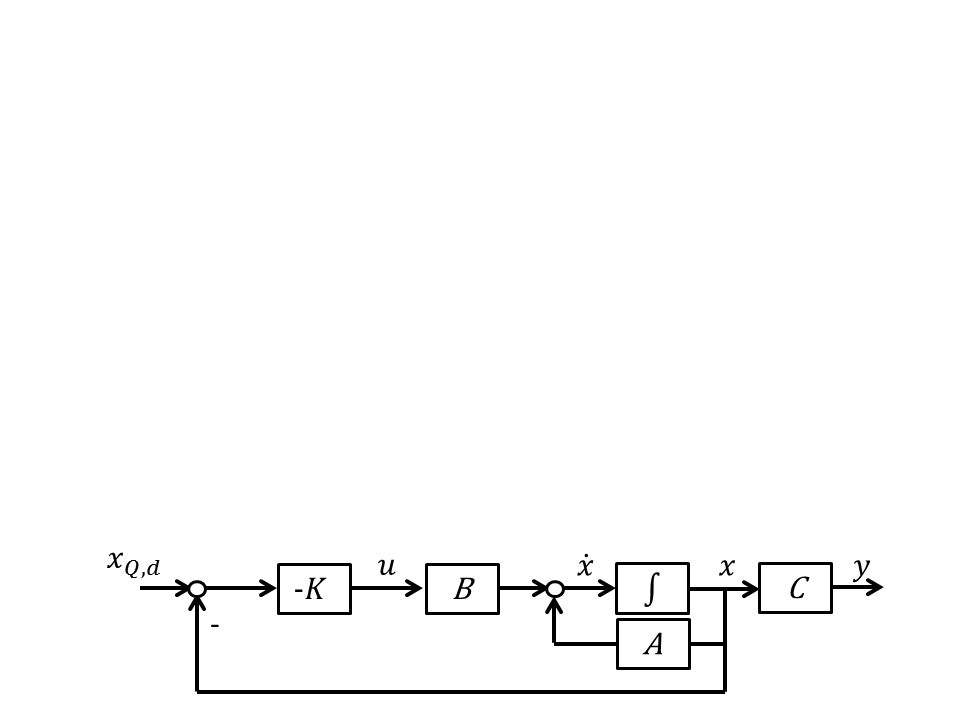
\includegraphics[trim={2cm 0 2cm 14cm},clip,width=.65\textwidth]{./StyleStuff/lqr.png}}
	\caption{LQR control design\label{fig:set.lqr}}
\end{figure}

\a{lqr} control is based on a small angle assumption. Therefore, a traditional modeling method may represent the rotation matrix with a local coordinate system, for example with an Euler Angle parameterization. 
A continuous time linearized model of the system used in this controller is represented in the following form 
\begin{align}\label{eq:ss}
\mathbf{\dot{x} }&=A\mathbf{x}+Bu\\
y&=C\mathbf{x}+Du
\end{align}
where $ \mathbf{x} $ is the state vector and $ u $ is the input vector, defined as follows
\begin{align}\label{eq:state}
%	\textbf{x}&=\begin{bmatrix}
%		\textbf{q}\\
%		\mathbf{\dot{q}}
%	\end{bmatrix}\\
%	\mathbf{q}&=\begin{bmatrix}
%		x&y&z&\phi&\theta&\psi&\phi_L&\theta_L
%	\end{bmatrix}^T\\
%	\mathbf{\dot{q}}&=\begin{bmatrix}
%		\dot{x}&\dot{y}&\dot{z}&\dot{\phi}&\dot{\theta}&\dot{\psi}&\dot{\phi}_L&\dot{\theta}_L
%	\end{bmatrix}^T\\
\mathbf{x}&=\begin{bmatrix}
x&y&z&\phi&\theta&\psi&\phi_L&\theta_L&\dot{x}&\dot{y}&\dot{z}&\dot{\phi}&\dot{\theta}&\dot{\psi}&\dot{\phi}_L&\dot{\theta}_L
\end{bmatrix}^T\\
u&=\begin{bmatrix}
f&M_\phi&M_\theta&M_\psi
\end{bmatrix}^T
\end{align}

Using \texttt{Matlab} command \texttt{lqr(A,B,Q,R)}, an optimal gain matrix $ K $ is calculated, such that the state-feedback law $ u=-K(\mathbf{x-x_{ref}}) $ minimizes the quadratic cost function \cite{Reyes-Valeria2013}. Where the cost function is defined as 
\begin{equation}\label{key}
J(u)=\int_{0}^{\infty}(\mathbf{x}^TQ\mathbf{x}+u^TRu)dt
\end{equation}
%where $ Q $ and $ R $ denote weight matrices that penalize the states and inputs in the cost function. 
The weight matrices $ Q $ and $ R $ that define the effects of the states and inputs in the cost function, and the gain matrix $K $ can be calculated. 
The derivation of the state space matrices $ A, B, C, D $, the weight matrices $ Q,R $ and the calculated gain matrix $ K $ can be found in Section \ref{app:lqr}. 

\newpage
\section{Results}\label{sec:exp.results}
In this section the results of the experiments are discussed.\\
In Figures \ref{fig:set.caseAres}, \ref{fig:set.caseBres} and \ref{fig:set.caseCres} the load tracking performance is shown for the Nonlinear Geometric Controller. 
The desired and actual load trajectories are show, and the corresponding load position errors are shown. \\
Figures \ref{fig:set.caseAres2}, \ref{fig:set.caseBres2} and \ref{fig:set.caseCres2} show the configuration errors $ \Psi_R, \Psi_q $, furthermore the corresponding tracking errors of the \a{qr} attitude $ e_R, e_\Omega $, load attitude $ e_q, e_{\dot{q}} $ and load position $ e_x,e_v $ are shown.
These results are analyzed to conclude stability of the system.\\
Figures \ref{fig:set.caseAres3}, \ref{fig:set.caseBres3} and \ref{fig:set.caseCres3} show the differences in controller performance between the Nonlinear Geometric Controller and the \a{lqr}. 

\subsection*{Case A}
In this case, the desired trajectory was shaped like a smooth step-like function to investigate the response of the system to a sudden input.
The desired and actual load trajectory, and the position error are shown in Figure \ref{fig:AxL} and Figure \ref{fig:AexL}, respectively.
It can be observed that the system responds with approximately $ 10 \% $ overshoot in the y-direction, while losing some height during this maneuver. 
Eventually the system stabilizes, and reaches a steady state.

\begin{figure}[h!]
	\centering
	\makebox[.49\textwidth][c]{\subfloat[][]{\includegraphics[trim={0.5cm 0 0.5cm 0},clip,width=.5\textwidth]{\dir{LPOSQRL-xL\caseA}}\label{fig:AxL}}}	
	\makebox[.49\textwidth][c]{\subfloat[][]{\includegraphics[trim={0.5cm 0 0.5cm 0},clip,width=.5\textwidth]{\dir{LPOSQRL-exL\caseA}}\label{fig:AexL}}}	
	\caption{Trajectory Tracking Nonlinear Geometric Control Case A \label{fig:set.caseAres}}
\end{figure}	

$ (e_x,e_v)=(0,0) $ is exponentially attractive. 

Figure \ref{fig:AeR} and \ref{fig:Aeq} show the tracking errors of the \a{qr} attitude and load attitude, respectively.\\
Observations: $(e_x,e_v,e_q,e_{\dot{q}},e_R,e_\Omega)=(0,0,0,0,0,0) $ is exponentially stable

Figure \ref{fig:APsiR} and \ref{fig:APsiq} show the tracking error functions of the \a{qr} and load, respectively. \\
Observations: there exist constants $ \alpha_q,\beta_q>0 $ such that
\begin{equation}\label{key}
\Psi_q(q(t),q_d(t)) \leq min\left\lbrace 2,\alpha_qe^{-\beta_qt}\right\rbrace 
\end{equation}
\begin{figure}[h!]
	\centering
	\makebox[.49\textwidth][c]{\subfloat[][]{\includegraphics[trim={0.5cm 0 0.5cm 0},clip,width=.5\textwidth]{\dir{LPOSQRL-eR\caseA}}\label{fig:AeR}}}	
	\makebox[.49\textwidth][c]{\subfloat[][]{\includegraphics[trim={0.5cm 0 0.5cm 0},clip,width=.5\textwidth]{\dir{LPOSQRL-eq\caseA}}\label{fig:Aeq}}}	
	\makebox[.49\textwidth][c]{\subfloat[][]{\includegraphics[trim={0.5cm 0 0.5cm 0},clip,width=.5\textwidth]{\dir{LPOSQRL-PsiR\caseA}}\label{fig:APsiR}}}
	\makebox[.49\textwidth][c]{\subfloat[][]{\includegraphics[trim={0.5cm 0 0.5cm 0},clip,width=.5\textwidth]{\dir{LPOSQRL-Psiq\caseA}}\label{fig:APsiq}}}
	\caption{Geometric Error functions Nonlinear Geometric Control Case A \label{fig:set.caseAres2}}
\end{figure}	

Figure \ref{fig:AxLlqr} shows the load position along the desired load position $ x_{L,d} $ for both control approaches.\\
Figure \ref{fig:AexLlqr} shows the load position error for both control approaches.
Figure \ref{fig:AQRang} shows the \a{qr} attitude with respect to \IF.\\
In Figure \ref{fig:ALang} the load angle with respect to \BF is shown.\\

\begin{figure}[p]
	\centering
	\makebox[.75\textwidth][c]{\subfloat[][Load position tracking \label{fig:AxLlqr}]{\includegraphics[width=.65\textwidth]{\dir{LQR-xL\caseA}}}}
	\makebox[.49\textwidth][c]{\subfloat[][QR Attitude\label{fig:AQRang}]{\includegraphics[trim={0.5cm 0 0.5cm 0},clip,width=.525\textwidth]{\dir{LQR-QRang\caseA}}}}
	\makebox[.49\textwidth][l]{\subfloat[][Load Attitude\label{fig:ALang}]{\includegraphics[trim={0.5cm 0 0.5cm 0},clip,width=.525\textwidth]{\dir{LQR-Lang\caseA}}}}
	\makebox[.49\textwidth][c]{\subfloat[][Load Position Error\label{fig:AexLlqr}]{\includegraphics[trim={0.5cm 0 0.5cm 0},clip,width=.525\textwidth]{\dir{LQR-exL\caseA}}}}	
	\caption{Controller Comparison Case A\label{fig:set.caseAres3}}	
\end{figure}
\clearpage

\newpage
\subsection*{Case B}
Figure \ref{fig:BxLlqr} shows the load position along the desired load position $ x_{L,d} $ of both controllers.

\begin{figure}[h!]
	\centering
	\makebox[.49\textwidth][c]{\subfloat[][]{\includegraphics[trim={0.5cm 0 0.5cm 0},clip,width=.5\textwidth]{\dir{LPOSQRL-xL\caseB}}\label{fig:BxL}}}	
	\makebox[.49\textwidth][c]{\subfloat[][]{\includegraphics[trim={0.5cm 0 0.5cm 0},clip,width=.5\textwidth]{\dir{LPOSQRL-exL\caseB}}\label{fig:BexL}}}	
	\caption{Trajectory Tracking Nonlinear Geometric Control Case B \label{fig:set.caseBres}}
\end{figure}	

\begin{figure}[h!]
	\centering
	\makebox[.49\textwidth][c]{\subfloat[][]{\includegraphics[trim={0.5cm 0 0.5cm 0},clip,width=.5\textwidth]{\dir{LPOSQRL-eR\caseB}}\label{fig:BeR}}}
    \makebox[.49\textwidth][c]{\subfloat[][]{\includegraphics[trim={0.5cm 0 0.5cm 0},clip,width=.5\textwidth]{\dir{LPOSQRL-eq\caseB}}\label{fig:Beq}}}	
	\makebox[.49\textwidth][c]{\subfloat[][]{\includegraphics[trim={0.5cm 0 0.5cm 0},clip,width=.5\textwidth]{\dir{LPOSQRL-PsiR\caseB}}\label{fig:BPsiR}}}
	\makebox[.49\textwidth][c]{\subfloat[][]{\includegraphics[trim={0.5cm 0 0.5cm 0},clip,width=.5\textwidth]{\dir{LPOSQRL-Psiq\caseB}}\label{fig:BPsiq}}}
	\caption{Geometric Error functions Nonlinear Geometric Control Case B \label{fig:set.caseBres2}}
\end{figure}	

Figure \ref{fig:BxLlqr} shows the load position along the desired load position $ x_{L,d} $ for both control approaches.\\
Figure \ref{fig:BexLlqr} shows the load position error for both control approaches.

\begin{figure}[h!]
	\centering
	\makebox[.75\textwidth][c]{\subfloat[][Load position tracking \label{fig:BxLlqr}]{\includegraphics[width=.65\textwidth]{\dir{LQR-xL\caseB}}}}
	\makebox[.49\textwidth][c]{\subfloat[][QR Attitude\label{fig:BQRang}]{\includegraphics[trim={0.5cm 0 0.5cm 0},clip,width=.525\textwidth]{\dir{LQR-QRang\caseB}}}}
	\makebox[.49\textwidth][l]{\subfloat[][Load Attitude\label{fig:BLang}]{\includegraphics[trim={0.5cm 0 0.5cm 0},clip,width=.525\textwidth]{\dir{LQR-Lang\caseB}}}}
	\makebox[.49\textwidth][c]{\subfloat[][Load Position Error\label{fig:BexLlqr}]{\includegraphics[trim={0.5cm 0 0.5cm 0},clip,width=.525\textwidth]{\dir{LQR-exL\caseB}}}}	
	\caption{Controller Comparison Case B\label{fig:set.caseBres3}}
\end{figure}	
\clearpage

\newpage
\subsection*{Case C}

Figure \ref{fig:CxLlqr} shows the load position along the desired load position $ x_{L,d} $ of both controllers.\\
Figure \ref{fig:CexLlqr} shows the load position error for both control approaches.\\
Observations: fact that LQR can not control load position is obvious.\\
OTHER GAINS FOR LQR!\\
Very small penalty on load angle results in swinging load; decreasing load position error, but very bad anti-swing. 

Figure \ref{fig:CQRang} shows the \a{qr} attitude with respect to \IF.\\
In Figure \ref{fig:CLang} the load angle with respect to \BF is shown. \\
Observations: Load angles are huge, check results

While tracking the required \a{qr} attitude, which tilts the \a{qr} to reach the desired velocities in the right direction, it can be seen that the system has difficulties to also maintain the desired height, which can be explained by the fact that the total force will not point upwards if the \a{qr} is tilted. Despite the fact that the \a{qr} is  moving from side to side, the upward force is still controlled to track the desired height. 

Figure \ref{fig:CxL} shows the desired load position, and Figure \ref{fig:CexL} shows that the error is mainly the overshoot in the x-direction, due to the fast desired swinging motion. 

Figure \ref{fig:CeR} and \ref{fig:Ceq} show the tracking errors of the \a{qr} attitude and load attitude, respectively. \\
Observations: $(e_x,e_v,e_q,e_{\dot{q}},e_R,e_\Omega)=(0,0,0,0,0,0) $ is exponentially stable

Figure \ref{fig:CPsiR} and \ref{fig:CPsiq} show the tracking error functions of the \a{qr} and load, respectively. \\
Observations: there exist constants $ \alpha_q,\beta_q>0 $ such that
\begin{equation}\label{key}
\Psi_q(q(t),q_d(t)) \leq min\left\lbrace 2,\alpha_qe^{-\beta_qt}\right\rbrace 
\end{equation}

\begin{figure}[h!]
	\centering
	\makebox[.49\textwidth][c]{\subfloat[][]{\includegraphics[trim={0.5cm 0 0.5cm 0},clip,width=.5\textwidth]{\dir{LPOSQRL-xL\caseC}}\label{fig:CxL}}}	
	\makebox[.49\textwidth][c]{\subfloat[][]{\includegraphics[trim={0.5cm 0 0.5cm 0},clip,width=.5\textwidth]{\dir{LPOSQRL-exL\caseC}}\label{fig:CexL}}}	
	\caption{Trajectory Tracking Nonlinear Geometric Control Case C \label{fig:set.caseCres}}
\end{figure}	

\begin{figure}[h!]
	\centering
	\makebox[.49\textwidth][c]{\subfloat[][]{\includegraphics[trim={0.5cm 0 0.5cm 0},clip,width=.5\textwidth]{\dir{LPOSQRL-eR\caseC}}\label{fig:CeR}}}
	\makebox[.49\textwidth][c]{\subfloat[][]{\includegraphics[trim={0.5cm 0 0.5cm 0},clip,width=.5\textwidth]{\dir{LPOSQRL-eq\caseC}}\label{fig:Ceq}}}	
	\makebox[.49\textwidth][c]{\subfloat[][]{\includegraphics[trim={0.5cm 0 0.5cm 0},clip,width=.5\textwidth]{\dir{LPOSQRL-PsiR\caseC}}\label{fig:CPsiR}}}
	\makebox[.49\textwidth][c]{\subfloat[][]{\includegraphics[trim={0.5cm 0 0.5cm 0},clip,width=.5\textwidth]{\dir{LPOSQRL-Psiq\caseC}}\label{fig:CPsiq}}}
	\caption{Geometric Error functions Nonlinear Geometric Control Case C \label{fig:set.caseCres2}}
\end{figure}	

Figure \ref{fig:CxLlqr} shows the load position along the desired load position $ x_{L,d} $ for both control approaches.\\
Figure \ref{fig:CexLlqr} shows the load position error for both control approaches.


\begin{figure}[h!]
	\centering
	\makebox[.75\textwidth][c]{\subfloat[][Load position tracking \label{fig:CxLlqr}]{\includegraphics[width=.65\textwidth]{\dir{LQR-xL\caseC}}}}
	\makebox[.49\textwidth][c]{\subfloat[][QR Attitude\label{fig:CQRang}]{\includegraphics[trim={0.5cm 0 0.5cm 0},clip,width=.525\textwidth]{\dir{LQR-QRang\caseC}}}}
	\makebox[.49\textwidth][l]{\subfloat[][Load Attitude\label{fig:CLang}]{\includegraphics[trim={0.5cm 0 0.5cm 0},clip,width=.525\textwidth]{\dir{LQR-Lang\caseC}}}}
	\makebox[.49\textwidth][c]{\subfloat[][Load Position Error\label{fig:CexLlqr}]{\includegraphics[trim={0.5cm 0 0.5cm 0},clip,width=.525\textwidth]{\dir{LQR-exL\caseC}}}}
	\caption{Controller Comparison Case C\label{fig:set.caseCres3}}
\end{figure}	
\clearpage

\newpage
\section{Conclusion}\label{set:exp.con}
%CHECK 
%What can we learn and conclude from different performance comparisons
%CHECK
%What is its value of nonlinear control compared to linear control

Near the equilibrium configuration, the \a{lqr} controller is able to reduce the swing. In fast trajectories however, the shortcomings of the \a{lqr} controller become evident. 

The nonlinear geometric controller depends on feed forward terms that are obtained from the desired trajectories. 
Trajectory generation approaches exist that are able to generate the required desired position, velocity and acceleration by 
however it is possible to compute these with trajectory generating algorithms too.

The controllers are functions of the computed tracking references $ q_c, R_c $ and their derivatives. These terms are approximated by a command filter, which means that the accuracy decreases because high frequency terms are filtered.

%CHECK
%It can be expected that the nonlinear geometric control allows large \a{qr} angles, whereas the \a{lqr} will possible fail to deviate far from the equilibrium point. 


%ADD conclusie 
% over parameter keuze in controllers. Arbitrair, maar wellicht later wel van belang



